\documentclass[10pt,a4paper,twocolumn]{article}

% ===== Paquetes básicos =====
\usepackage[spanish]{babel}      
\usepackage[utf8]{inputenc}      
\usepackage[T1]{fontenc}         
\usepackage{amsmath, amssymb}    
\usepackage{graphicx}            
\usepackage{float}               
\usepackage{siunitx}             
\usepackage{tikz}                
\usepackage{circuitikz}
\usepackage{caption}             
\usepackage{geometry}
\usepackage{stfloats}
\usepackage{mhchem}
\usepackage{booktabs}
\usepackage[hyphens]{url}
\usepackage{hyperref}
\usepackage{subcaption}
\usepackage{physics}
\urlstyle{same}
\geometry{top=2cm,bottom=2cm,left=2cm,right=2cm}
\usepackage{tocloft}
% Texto del índice normal, sin negritas en números
\renewcommand{\cftsecfont}{\normalfont}
\renewcommand{\cftsecpagefont}{\normalfont}

\DeclareSIUnit{\calorie}{cal}
\sisetup{
    output-decimal-marker = {,},
    separate-uncertainty = true,  % Esto muestra ± en lugar de ()
    uncertainty-separator = {\,\pm\,}
}

% ===== Estilo de captions =====
\captionsetup[figure]{labelfont=bf}
\captionsetup[table]{labelfont=bf, name=Tabla}

% ===== Palabras clave =====
\newcommand{\keywords}[1]{\vspace{2mm}\noindent\textbf{Palabras clave:} #1}

% ===== Títulos de secciones =====
\usepackage{sectsty}
%\allsectionsfont{\centering\uppercase}
\sectionfont{\centering\normalsize\uppercase}
\subsectionfont{\centering\small\uppercase}
\subsubsectionfont{\centering\small\itshape}
\renewcommand{\thesection}{\Roman{section}}

% ===== Datos del informe (centrado) =====
\title{\textbf{\LARGE TODO}}
\author{
\large Francisco Utrera - Facundo Picco\\[2mm]
\small \textit{Informe de Experimental II -- Instituto Balseiro} \\
\small \textit{Universidad Nacional de Cuyo \& Comisión Nacional de Energía Atómica} \\
\small \textit{Av. Bustillo 9500, c.p.8400 San Carlos de Bariloche, Río Negro, Argentina} \\
\small \texttt{francisco.utrera@ib.edu.ar} \texttt{facundo.picco@ib.edu.ar} %tu mail khalid
}
\date{\today}

\begin{document}

% ===== Portada =====
\twocolumn[
\begin{@twocolumnfalse}
    \maketitle
    \begin{abstract}
    TODO
    \end{abstract}
    \keywords{}
    \vspace{1cm}
\end{@twocolumnfalse}
]


% ===== Secciones =====

\section{Introducción}
Según Antonoff \cite{cristal_def}, un cristal es un cuerpo homogéneo anisotrópico que tiene la forma natural de un poliedro. Estos están compuestos por átomos
o grupos de estos, organizados en patrones periódicos en tres dimensiones.

Para describir dichos cristales es útil pensar al cristal como una red de puntos, de manera que cada punto represente la posición de un átomo, como se observa en la Figura \ref{fig: red_cristalina}:

\begin{figure}[!h]
    \centering
    

\tikzset{every picture/.style={line width=0.75pt}} %set default line width to 0.75pt        

\begin{tikzpicture}[x=0.75pt,y=0.75pt,yscale=-.9,xscale=.9]
%uncomment if require: \path (0,300); %set diagram left start at 0, and has height of 300

%Shape: Parallelogram [id:dp00009525685621813995] 
\draw  [line width=1.5]  (156,165) -- (205,165) -- (184,205) -- (135,205) -- cycle ;
%Shape: Parallelogram [id:dp971726964278922] 
\draw  [line width=0.75]  (205,165) -- (254,165) -- (233,205) -- (184,205) -- cycle ;
%Shape: Parallelogram [id:dp9953454360121382] 
\draw  [line width=0.75]  (254,165) -- (303,165) -- (282,205) -- (233,205) -- cycle ;
%Shape: Parallelogram [id:dp40940416939952784] 
\draw  [line width=0.75]  (177,125) -- (226,125) -- (205,165) -- (156,165) -- cycle ;
%Shape: Parallelogram [id:dp7691692691036712] 
\draw  [line width=0.75]  (226,125) -- (275,125) -- (254,165) -- (205,165) -- cycle ;
%Shape: Parallelogram [id:dp6917201527235944] 
\draw  [line width=0.75]  (275,125) -- (324,125) -- (303,165) -- (254,165) -- cycle ;
%Shape: Parallelogram [id:dp09548041083729841] 
\draw  [line width=0.75]  (198,85) -- (247,85) -- (226,125) -- (177,125) -- cycle ;
%Shape: Parallelogram [id:dp904852767837213] 
\draw  [line width=0.75]  (247,85) -- (296,85) -- (275,125) -- (226,125) -- cycle ;
%Shape: Parallelogram [id:dp7317550277246561] 
\draw  [line width=0.75]  (296,85) -- (345,85) -- (324,125) -- (275,125) -- cycle ;
%Shape: Parallelogram [id:dp8092966968757053] 
\draw  [line width=1.5]  (184.21,187.9) -- (233.21,187.9) -- (184,205) -- (135,205) -- cycle ;
%Shape: Parallelogram [id:dp5589381507177117] 
\draw  [line width=0.75]  (233.21,187.9) -- (282.21,187.9) -- (233,205) -- (184,205) -- cycle ;
%Shape: Parallelogram [id:dp2926331891595425] 
\draw  [line width=0.75]  (282.21,187.9) -- (331.21,187.9) -- (282,205) -- (233,205) -- cycle ;
%Shape: Parallelogram [id:dp042729226133859766] 
\draw  [line width=1.5]  (205.21,147.9) -- (254.21,147.9) -- (205,165) -- (156,165) -- cycle ;
%Shape: Parallelogram [id:dp9849438978419048] 
\draw  [line width=0.75]  (254.21,147.9) -- (303.21,147.9) -- (254,165) -- (205,165) -- cycle ;
%Shape: Parallelogram [id:dp7410971278074631] 
\draw  [line width=1.5]  (303.21,147.9) -- (352.21,147.9) -- (303,165) -- (254,165) -- cycle ;
%Shape: Parallelogram [id:dp10478652077359119] 
\draw  [line width=0.75]  (247.21,67.9) -- (296.21,67.9) -- (247,85) -- (198,85) -- cycle ;
%Shape: Parallelogram [id:dp9671189751149326] 
\draw  [line width=0.75]  (296.21,67.9) -- (345.21,67.9) -- (296,85) -- (247,85) -- cycle ;
%Shape: Parallelogram [id:dp7462215561963487] 
\draw  [line width=0.75]  (345.21,67.9) -- (394.21,67.9) -- (345,85) -- (296,85) -- cycle ;
%Straight Lines [id:da3244862013467892] 
\draw [line width=1.5]    (184.21,187.9) -- (205.21,147.9) ;
%Straight Lines [id:da9079694089980225] 
\draw [line width=1.5]    (233.21,187.9) -- (254.21,147.9) ;
%Straight Lines [id:da8989243244205052] 
\draw [line width=0.75]    (282.21,187.9) -- (345.21,67.9) ;
%Straight Lines [id:da509334709094928] 
\draw [line width=0.75]    (331.21,187.9) -- (394.21,67.9) ;
%Shape: Parallelogram [id:dp20749812905199472] 
\draw  [line width=0.75]  (226.21,107.9) -- (275.21,107.9) -- (226,125) -- (177,125) -- cycle ;
%Shape: Parallelogram [id:dp5486843238595097] 
\draw  [line width=1.5]  (275.21,107.9) -- (324.21,107.9) -- (275,125) -- (226,125) -- cycle ;
%Shape: Parallelogram [id:dp16023221231370466] 
\draw  [line width=0.75]  (324.21,107.9) -- (373.21,107.9) -- (324,125) -- (275,125) -- cycle ;
%Shape: Circle [id:dp590508497504874] 
\draw  [fill={rgb, 255:red, 0; green, 0; blue, 0 }  ,fill opacity=1 ] (154.08,165) .. controls (154.08,163.94) and (154.94,163.08) .. (156,163.08) .. controls (157.06,163.08) and (157.92,163.94) .. (157.92,165) .. controls (157.92,166.06) and (157.06,166.92) .. (156,166.92) .. controls (154.94,166.92) and (154.08,166.06) .. (154.08,165) -- cycle ;
%Shape: Circle [id:dp4365962359814469] 
\draw  [fill={rgb, 255:red, 0; green, 0; blue, 0 }  ,fill opacity=1 ] (133.08,205) .. controls (133.08,203.94) and (133.94,203.08) .. (135,203.08) .. controls (136.06,203.08) and (136.92,203.94) .. (136.92,205) .. controls (136.92,206.06) and (136.06,206.92) .. (135,206.92) .. controls (133.94,206.92) and (133.08,206.06) .. (133.08,205) -- cycle ;
%Shape: Circle [id:dp6835008947696789] 
\draw  [fill={rgb, 255:red, 0; green, 0; blue, 0 }  ,fill opacity=1 ] (182.08,205) .. controls (182.08,203.94) and (182.94,203.08) .. (184,203.08) .. controls (185.06,203.08) and (185.92,203.94) .. (185.92,205) .. controls (185.92,206.06) and (185.06,206.92) .. (184,206.92) .. controls (182.94,206.92) and (182.08,206.06) .. (182.08,205) -- cycle ;
%Shape: Circle [id:dp494641160799808] 
\draw  [fill={rgb, 255:red, 0; green, 0; blue, 0 }  ,fill opacity=1 ] (203.08,165) .. controls (203.08,163.94) and (203.94,163.08) .. (205,163.08) .. controls (206.06,163.08) and (206.92,163.94) .. (206.92,165) .. controls (206.92,166.06) and (206.06,166.92) .. (205,166.92) .. controls (203.94,166.92) and (203.08,166.06) .. (203.08,165) -- cycle ;
%Shape: Circle [id:dp4247274346041169] 
\draw  [fill={rgb, 255:red, 0; green, 0; blue, 0 }  ,fill opacity=1 ] (175.08,125) .. controls (175.08,123.94) and (175.94,123.08) .. (177,123.08) .. controls (178.06,123.08) and (178.92,123.94) .. (178.92,125) .. controls (178.92,126.06) and (178.06,126.92) .. (177,126.92) .. controls (175.94,126.92) and (175.08,126.06) .. (175.08,125) -- cycle ;
%Shape: Circle [id:dp42134666221625616] 
\draw  [fill={rgb, 255:red, 0; green, 0; blue, 0 }  ,fill opacity=1 ] (224.08,125) .. controls (224.08,123.94) and (224.94,123.08) .. (226,123.08) .. controls (227.06,123.08) and (227.92,123.94) .. (227.92,125) .. controls (227.92,126.06) and (227.06,126.92) .. (226,126.92) .. controls (224.94,126.92) and (224.08,126.06) .. (224.08,125) -- cycle ;
%Shape: Circle [id:dp2055200872359486] 
\draw  [fill={rgb, 255:red, 0; green, 0; blue, 0 }  ,fill opacity=1 ] (231.08,205) .. controls (231.08,203.94) and (231.94,203.08) .. (233,203.08) .. controls (234.06,203.08) and (234.92,203.94) .. (234.92,205) .. controls (234.92,206.06) and (234.06,206.92) .. (233,206.92) .. controls (231.94,206.92) and (231.08,206.06) .. (231.08,205) -- cycle ;
%Shape: Circle [id:dp14873206132643946] 
\draw  [fill={rgb, 255:red, 0; green, 0; blue, 0 }  ,fill opacity=1 ] (252.08,165) .. controls (252.08,163.94) and (252.94,163.08) .. (254,163.08) .. controls (255.06,163.08) and (255.91,163.94) .. (255.91,165) .. controls (255.91,166.06) and (255.06,166.92) .. (254,166.92) .. controls (252.94,166.92) and (252.08,166.06) .. (252.08,165) -- cycle ;
%Shape: Circle [id:dp07697785152375225] 
\draw  [fill={rgb, 255:red, 0; green, 0; blue, 0 }  ,fill opacity=1 ] (280.08,205) .. controls (280.08,203.94) and (280.94,203.08) .. (282,203.08) .. controls (283.06,203.08) and (283.92,203.94) .. (283.92,205) .. controls (283.92,206.06) and (283.06,206.92) .. (282,206.92) .. controls (280.94,206.92) and (280.08,206.06) .. (280.08,205) -- cycle ;
%Shape: Circle [id:dp47549778776945495] 
\draw  [fill={rgb, 255:red, 0; green, 0; blue, 0 }  ,fill opacity=1 ] (301.08,165) .. controls (301.08,163.94) and (301.94,163.08) .. (303,163.08) .. controls (304.05,163.08) and (304.91,163.94) .. (304.91,165) .. controls (304.91,166.06) and (304.05,166.92) .. (303,166.92) .. controls (301.94,166.92) and (301.08,166.06) .. (301.08,165) -- cycle ;
%Shape: Circle [id:dp40074665187916125] 
\draw  [fill={rgb, 255:red, 0; green, 0; blue, 0 }  ,fill opacity=1 ] (182.3,187.9) .. controls (182.3,186.84) and (183.16,185.98) .. (184.21,185.98) .. controls (185.27,185.98) and (186.13,186.84) .. (186.13,187.9) .. controls (186.13,188.96) and (185.27,189.82) .. (184.21,189.82) .. controls (183.16,189.82) and (182.3,188.96) .. (182.3,187.9) -- cycle ;
%Shape: Circle [id:dp5871823356343124] 
\draw  [fill={rgb, 255:red, 0; green, 0; blue, 0 }  ,fill opacity=1 ] (231.3,187.9) .. controls (231.3,186.84) and (232.16,185.98) .. (233.21,185.98) .. controls (234.27,185.98) and (235.13,186.84) .. (235.13,187.9) .. controls (235.13,188.96) and (234.27,189.82) .. (233.21,189.82) .. controls (232.16,189.82) and (231.3,188.96) .. (231.3,187.9) -- cycle ;
%Shape: Circle [id:dp827870478136313] 
\draw  [fill={rgb, 255:red, 0; green, 0; blue, 0 }  ,fill opacity=1 ] (280.3,187.9) .. controls (280.3,186.84) and (281.16,185.98) .. (282.21,185.98) .. controls (283.27,185.98) and (284.13,186.84) .. (284.13,187.9) .. controls (284.13,188.96) and (283.27,189.82) .. (282.21,189.82) .. controls (281.16,189.82) and (280.3,188.96) .. (280.3,187.9) -- cycle ;
%Shape: Circle [id:dp726496781868341] 
\draw  [fill={rgb, 255:red, 0; green, 0; blue, 0 }  ,fill opacity=1 ] (329.3,187.9) .. controls (329.3,186.84) and (330.15,185.98) .. (331.21,185.98) .. controls (332.27,185.98) and (333.13,186.84) .. (333.13,187.9) .. controls (333.13,188.96) and (332.27,189.82) .. (331.21,189.82) .. controls (330.15,189.82) and (329.3,188.96) .. (329.3,187.9) -- cycle ;
%Shape: Circle [id:dp1869487666588726] 
\draw  [fill={rgb, 255:red, 0; green, 0; blue, 0 }  ,fill opacity=1 ] (350.29,147.9) .. controls (350.29,146.84) and (351.15,145.98) .. (352.21,145.98) .. controls (353.27,145.98) and (354.13,146.84) .. (354.13,147.9) .. controls (354.13,148.96) and (353.27,149.82) .. (352.21,149.82) .. controls (351.15,149.82) and (350.29,148.96) .. (350.29,147.9) -- cycle ;
%Shape: Circle [id:dp6347726644456305] 
\draw  [fill={rgb, 255:red, 0; green, 0; blue, 0 }  ,fill opacity=1 ] (301.29,147.9) .. controls (301.29,146.84) and (302.15,145.98) .. (303.21,145.98) .. controls (304.27,145.98) and (305.13,146.84) .. (305.13,147.9) .. controls (305.13,148.96) and (304.27,149.82) .. (303.21,149.82) .. controls (302.15,149.82) and (301.29,148.96) .. (301.29,147.9) -- cycle ;
%Shape: Circle [id:dp013051651080519533] 
\draw  [fill={rgb, 255:red, 0; green, 0; blue, 0 }  ,fill opacity=1 ] (252.29,147.9) .. controls (252.29,146.84) and (253.15,145.98) .. (254.21,145.98) .. controls (255.27,145.98) and (256.13,146.84) .. (256.13,147.9) .. controls (256.13,148.96) and (255.27,149.82) .. (254.21,149.82) .. controls (253.15,149.82) and (252.29,148.96) .. (252.29,147.9) -- cycle ;
%Shape: Circle [id:dp4030775579990349] 
\draw  [fill={rgb, 255:red, 0; green, 0; blue, 0 }  ,fill opacity=1 ] (203.3,147.9) .. controls (203.3,146.84) and (204.15,145.98) .. (205.21,145.98) .. controls (206.27,145.98) and (207.13,146.84) .. (207.13,147.9) .. controls (207.13,148.96) and (206.27,149.82) .. (205.21,149.82) .. controls (204.15,149.82) and (203.3,148.96) .. (203.3,147.9) -- cycle ;
%Shape: Circle [id:dp7226979973133509] 
\draw  [fill={rgb, 255:red, 0; green, 0; blue, 0 }  ,fill opacity=1 ] (224.3,107.9) .. controls (224.3,106.84) and (225.16,105.98) .. (226.21,105.98) .. controls (227.27,105.98) and (228.13,106.84) .. (228.13,107.9) .. controls (228.13,108.96) and (227.27,109.82) .. (226.21,109.82) .. controls (225.16,109.82) and (224.3,108.96) .. (224.3,107.9) -- cycle ;
%Shape: Circle [id:dp37231938913536766] 
\draw  [fill={rgb, 255:red, 0; green, 0; blue, 0 }  ,fill opacity=1 ] (273.3,107.9) .. controls (273.3,106.84) and (274.16,105.98) .. (275.21,105.98) .. controls (276.27,105.98) and (277.13,106.84) .. (277.13,107.9) .. controls (277.13,108.96) and (276.27,109.82) .. (275.21,109.82) .. controls (274.16,109.82) and (273.3,108.96) .. (273.3,107.9) -- cycle ;
%Shape: Circle [id:dp4743778777159975] 
\draw  [fill={rgb, 255:red, 0; green, 0; blue, 0 }  ,fill opacity=1 ] (273.08,125) .. controls (273.08,123.94) and (273.94,123.08) .. (275,123.08) .. controls (276.06,123.08) and (276.92,123.94) .. (276.92,125) .. controls (276.92,126.06) and (276.06,126.92) .. (275,126.92) .. controls (273.94,126.92) and (273.08,126.06) .. (273.08,125) -- cycle ;
%Shape: Circle [id:dp9131151792951618] 
\draw  [fill={rgb, 255:red, 0; green, 0; blue, 0 }  ,fill opacity=1 ] (322.08,125) .. controls (322.08,123.94) and (322.94,123.08) .. (324,123.08) .. controls (325.06,123.08) and (325.92,123.94) .. (325.92,125) .. controls (325.92,126.06) and (325.06,126.92) .. (324,126.92) .. controls (322.94,126.92) and (322.08,126.06) .. (322.08,125) -- cycle ;
%Shape: Circle [id:dp87642839600309] 
\draw  [fill={rgb, 255:red, 0; green, 0; blue, 0 }  ,fill opacity=1 ] (371.3,107.9) .. controls (371.3,106.84) and (372.15,105.98) .. (373.21,105.98) .. controls (374.27,105.98) and (375.13,106.84) .. (375.13,107.9) .. controls (375.13,108.96) and (374.27,109.82) .. (373.21,109.82) .. controls (372.15,109.82) and (371.3,108.96) .. (371.3,107.9) -- cycle ;
%Shape: Circle [id:dp7235571417857445] 
\draw  [fill={rgb, 255:red, 0; green, 0; blue, 0 }  ,fill opacity=1 ] (322.3,107.9) .. controls (322.3,106.84) and (323.15,105.98) .. (324.21,105.98) .. controls (325.27,105.98) and (326.13,106.84) .. (326.13,107.9) .. controls (326.13,108.96) and (325.27,109.82) .. (324.21,109.82) .. controls (323.15,109.82) and (322.3,108.96) .. (322.3,107.9) -- cycle ;
%Shape: Circle [id:dp07424531105449717] 
\draw  [fill={rgb, 255:red, 0; green, 0; blue, 0 }  ,fill opacity=1 ] (196.08,85) .. controls (196.08,83.94) and (196.94,83.08) .. (198,83.08) .. controls (199.06,83.08) and (199.92,83.94) .. (199.92,85) .. controls (199.92,86.06) and (199.06,86.92) .. (198,86.92) .. controls (196.94,86.92) and (196.08,86.06) .. (196.08,85) -- cycle ;
%Shape: Circle [id:dp24587126841829599] 
\draw  [fill={rgb, 255:red, 0; green, 0; blue, 0 }  ,fill opacity=1 ] (245.08,85) .. controls (245.08,83.94) and (245.94,83.08) .. (247,83.08) .. controls (248.06,83.08) and (248.92,83.94) .. (248.92,85) .. controls (248.92,86.06) and (248.06,86.92) .. (247,86.92) .. controls (245.94,86.92) and (245.08,86.06) .. (245.08,85) -- cycle ;
%Shape: Circle [id:dp29357273468241374] 
\draw  [fill={rgb, 255:red, 0; green, 0; blue, 0 }  ,fill opacity=1 ] (294.08,85) .. controls (294.08,83.94) and (294.94,83.08) .. (296,83.08) .. controls (297.06,83.08) and (297.92,83.94) .. (297.92,85) .. controls (297.92,86.06) and (297.06,86.92) .. (296,86.92) .. controls (294.94,86.92) and (294.08,86.06) .. (294.08,85) -- cycle ;
%Shape: Circle [id:dp31317366309255423] 
\draw  [fill={rgb, 255:red, 0; green, 0; blue, 0 }  ,fill opacity=1 ] (343.08,85) .. controls (343.08,83.94) and (343.94,83.08) .. (345,83.08) .. controls (346.06,83.08) and (346.92,83.94) .. (346.92,85) .. controls (346.92,86.06) and (346.06,86.92) .. (345,86.92) .. controls (343.94,86.92) and (343.08,86.06) .. (343.08,85) -- cycle ;
%Shape: Circle [id:dp24106233649331332] 
\draw  [fill={rgb, 255:red, 0; green, 0; blue, 0 }  ,fill opacity=1 ] (392.3,67.9) .. controls (392.3,66.84) and (393.15,65.98) .. (394.21,65.98) .. controls (395.27,65.98) and (396.13,66.84) .. (396.13,67.9) .. controls (396.13,68.96) and (395.27,69.82) .. (394.21,69.82) .. controls (393.15,69.82) and (392.3,68.96) .. (392.3,67.9) -- cycle ;
%Shape: Circle [id:dp8875098572588417] 
\draw  [fill={rgb, 255:red, 0; green, 0; blue, 0 }  ,fill opacity=1 ] (343.3,67.9) .. controls (343.3,66.84) and (344.16,65.98) .. (345.21,65.98) .. controls (346.27,65.98) and (347.13,66.84) .. (347.13,67.9) .. controls (347.13,68.96) and (346.27,69.82) .. (345.21,69.82) .. controls (344.16,69.82) and (343.3,68.96) .. (343.3,67.9) -- cycle ;
%Shape: Circle [id:dp9111714493949994] 
\draw  [fill={rgb, 255:red, 0; green, 0; blue, 0 }  ,fill opacity=1 ] (294.3,67.9) .. controls (294.3,66.84) and (295.16,65.98) .. (296.21,65.98) .. controls (297.27,65.98) and (298.13,66.84) .. (298.13,67.9) .. controls (298.13,68.96) and (297.27,69.82) .. (296.21,69.82) .. controls (295.16,69.82) and (294.3,68.96) .. (294.3,67.9) -- cycle ;
%Shape: Circle [id:dp45227619601882063] 
\draw  [fill={rgb, 255:red, 0; green, 0; blue, 0 }  ,fill opacity=1 ] (245.3,67.9) .. controls (245.3,66.84) and (246.16,65.98) .. (247.21,65.98) .. controls (248.27,65.98) and (249.13,66.84) .. (249.13,67.9) .. controls (249.13,68.96) and (248.27,69.82) .. (247.21,69.82) .. controls (246.16,69.82) and (245.3,68.96) .. (245.3,67.9) -- cycle ;
%Straight Lines [id:da38738734123248053] 
\draw [line width=0.75]    (205.22,147.9) -- (247.21,67.9) ;
%Straight Lines [id:da5261615357095674] 
\draw [line width=0.75]    (254.21,147.9) -- (296.21,67.9) ;
%Straight Lines [id:da24380223752871444] 
\draw [line width=1.5]    (226,125) -- (254,165) ;
%Straight Lines [id:da9984205950739007] 
\draw [line width=1.5]    (275.21,107.9) -- (303.21,147.9) ;
%Straight Lines [id:da3289383838858638] 
\draw [line width=1.5]    (275,125) -- (303,165) ;
%Straight Lines [id:da9482733584495318] 
\draw [line width=1.5]    (324.21,107.9) -- (352.21,147.9) ;




\end{tikzpicture}

\caption{Ejemplo de una red cristalina con celdas unidades remarcadas en negro.}
\label{fig: red_cristalina}

\end{figure}

Como se observa en la Figura \ref{fig: red_cristalina}, al unir los puntos de la red se forman celdas repetidas periódicamente a lo largo de esta. Dichas celdas se denominan celdas unidad y  la red es obtenida por repetición de dicha celda. En la Figura \ref{fig: red_cristalina} se muestra en remarcado en negro distintas celdas unidad posibles.
De esta forma la red queda definida al indicar las distancias entre puntos en tres direcciones y los ángulos entre estas. Dichas distancias y ángulos forman vectores llamados parámetros de red de la celda unidad. Cabe decir que hay solo 14 tipos de celdas unidad posibles, las llamadas redes de Bravais, ya que cualquier otra celda hallada es equivalente a una de estas 14.

Finalmente tenemos el motivo, que representa la distribución de los átomos en la celda unidad. Son el mínimo conjunto de átomos, iones o moléculas que se repiten. Así toda estructura cristalina puede representarse como su motivo más la red de Bravais correspondiente.

En el presente trabajo se tratarán cristales con estructura de tipo sal de roca, que consisten en una red de Bravais FCC (Face-Centered Cubic), cuyo motivo consta de un catión en la posición (0,0,0) y un anión en la posición (1/2, 1/2, 1/2), tal como se muestra en la Figura \ref{fig: celda_sal_roca},
donde los átomos amarillos representan los cationes y los verdes los aniones. Debido al tipo de red, basta con indicar un sólo parámetro de red, que se denotará por $a$.

\begin{figure}[!h]
\centering
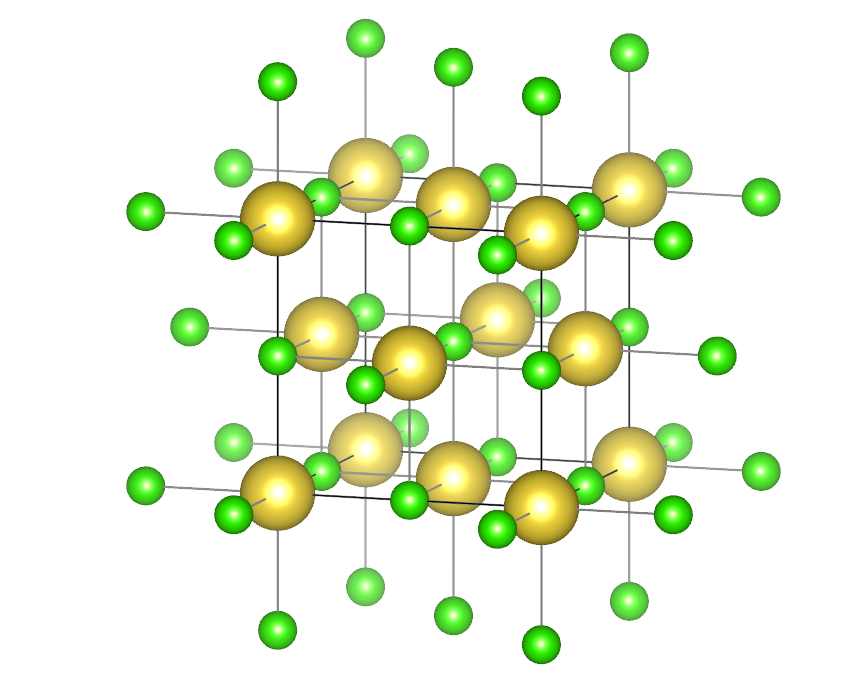
\includegraphics[width=.9\columnwidth]{Imagenes/1000041.png}
\caption{Celda unidad de un cristal con estructura de tipo sal de roca extraída con el programa VESTA.}
\label{fig: celda_sal_roca}
\end{figure}

Por otro lado, los puntos de red son intersecados por planos imaginarios que se denominan planos cristalinos. Para representar dichos planos se hace uso de la notación de Miller. Dicha
notación consiste en describir al plano mediante los recíprocos de las intersecciones del plano con los ejes coordenados a través de la notación (hkl).  Esto se muestra en la Figura \ref{fig: notacion_miller}

\begin{figure}[h]
\centering
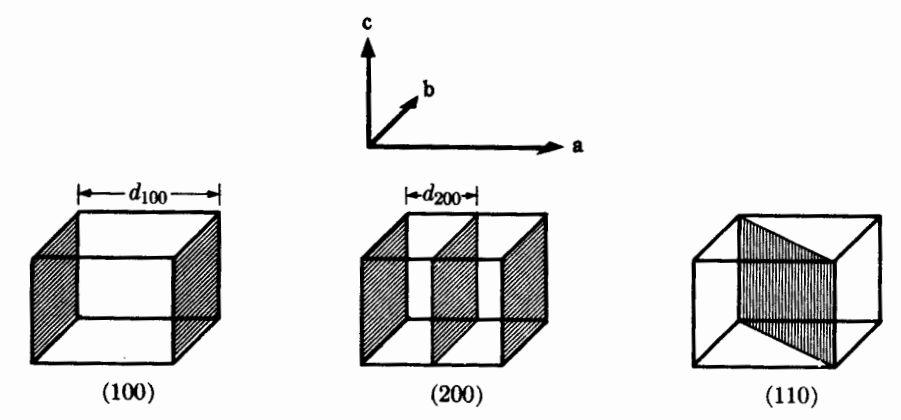
\includegraphics[width=\columnwidth]{Imagenes/planos miller.png}
\caption{Indices de Miller para distintos planos cristalinos, siendo $d$ la distancia interplanar. Extraído de \cite{cullity}.}
\label{fig: notacion_miller}
\end{figure}

Debido a la periodicidad de la red, los planos cristalinos se repiten también peródicamente. La distancia entre dos planos sucesivos se denomina distancia interplanar $d.$ En una red FCC, la distancia interplanar está dada por
\begin{equation}
    d_{hkl}=\frac{a}{\sqrt{h^2+k^2+l^2}},
\label{eq: distancia_interplanar}
\end{equation}

siendo $a$ el parámetro de red.

La ley de Bragg \cite{ley_bragg} establece que la difracción de rayos X en un cristal es constructiva si la diferencia de camino entre los rayos reflejados es un múltiplo entero de la longitud de onda. Esto se expresa como

\begin{equation}
    n\lambda=2d\sin\theta,
\label{eq: ley_bragg}
\end{equation}
siendo $\lambda$ la longitud de onda del rayo X, $d$ la distancia interplanar y $\theta$ el ángulo de incidencia. Algo importante es que la difracción ocurre si la longitud de onda es del orden de magnitud de la distancia interplanar.
De esta forma, al medir el ángulo $\theta$ de difracción y conociendo la longitud de onda, puede obtenerse la distancia interplanar $d$ por la Ecuación \ref{eq: ley_bragg}. Luego, si se determina a que plano (hkl) corresponde dicha distancia
interplanar, por la Ecuación \ref{eq: distancia_interplanar} puede obtenerse el parámetro de red $a.$

Para determinar a qué plano corresponde cada difracción constructiva se hace uso del factor de estructura. El cuadrado de dicho valor es proporcional a la intensidad de la difracción y es definido como

\begin{equation}
    F_{hkl}=\sum_{j=1}^{N}f_j e^{2\pi i \mathbf{r_j}\cdot (hkl)},
\label{eq: factor_estructura}
\end{equation}

donde $f_j$ es el factor atómico, proporcional al número atómico, $N$ la cantidad de átomos que forman la celda unidad y $\mathbf{r_j}$ la posición del átomo $j$ dentro de la celda unidad. De la Ecuación \ref{eq: factor_estructura}, en una red FCC con motivo de tipo sal de roca, el factor de estructura está dado por

\begin{equation}
    F_{hkl}=\begin{cases}
    4(f_{cat}+f_{an}) & \text{si } h,k,l \text{ son todos pares} \\
    4(f_{cat}-f_{an}) & \text{si } h,k,l \text{ son todos impares} \\
    0 & \text{en otro caso},
    \end{cases}
\end{equation}

donde $f_{cat}$ y $f_{an}$ son los factores atómicos del catión y el anión respectivamente. Como los factores atómicos son proporcionales al número átomico, en el caso de planos con índices impares, si los números atómicos son similares la intensidad medida es muy baja, lo que se denomina \textit{extinción sistemática de picos}.

La ley de Vegard \cite{Vegard1921} es una ley empírica que establece que en soluciones cristalinas sólidas el parámetro de red sigue una relación lineal con la concentración de los componentes:

\begin{equation}
    a = (1-x)a_A + xa_B,
\label{eq: ley_vegard}
\end{equation}

siendo $a$ el parámetro de red de la solución sólida, $a_A$ y $a_B$ los parámetros de red de los componentes puros A y B respectivamente, y $x$ la concentración del componente B. En este trabajo se busca verificar experimentalmente la validez de la Ecuación \ref{eq: ley_vegard}, además de analizar los difractogramas de distintas soluciones sólidas y compositos.

\section{Método experimental}
El experimento consistió en el uso de un difractómetro de rayos X \textit{BRUKER D2 PHASER}, en el cual se colocaba la muestra sólida sobre un portamuestras. En un principio, se realizó el barrido de la sal de mesa y la sal \textit{light}. 

Luego, se prepararon las muestras para las sales puras de KCl y KBr, así como sus soluciones. Estas últimas se formularon para distintos porcentajes molares, donde $X_{Br}$ representa la fracción molar de KBr y $X_{Cl} = 1 - X_{Br}$ la fracción molar de KCl. Las mezclas realizadas correspondieron a los siguientes porcentajes molares de KBr: 0\,\%, 20\,\%, 40\,\%, 60\,\% y 80\,\%.

Para la preparación de las soluciones, primero se colocaron las sales puras de KCl y KBr en vasos de precipitados y se calentaron durante aproximadamente 10 minutos sobre una platina calentadora. El objetivo de este paso fue evaporar la humedad residual que pudieran contener y así poder pesarlas con exactitud en una balanza de precisión (\textit{Insertar aquí el nombre de la balanza}) para obtener las proporciones molares deseadas. Una vez pesadas, las sales se combinaron en un vaso de precipitados y se disolvieron en agua destilada.

Las soluciones resultantes se dejaron reposar durante unos 5 días para permitir la evaporación del solvente y la posterior cocristalización. Como la evaporación natural no se completó debido a la humedad del ambiente, se aceleró el proceso colocando las muestras sobre una platina calentadora hasta evaporar la totalidad del agua, obteniendo así las muestras sólidas finales para su caracterización. Es importante destacar que la evaporación rápida del solvente no favorece un crecimiento cristalino ordenado, lo que dificulta la observación clara del proceso de cristalización en las muestras.

Adicionalmente, se preparó una solución pura de KBr mediante su disolución en agua destilada. Esta muestra se dejó evaporar a temperatura ambiente durante más de una semana con el objetivo de promover un crecimiento lento, obteniendo así cristales más grandes y ordenados que permitieran observar el proceso de cristalización con mayor claridad.

El equipo opera en geometría Bragg--Brentano, en la cual la muestra se encuentra en el centro del goniómetro y el sistema realiza un barrido $\theta$--$2\theta$, manteniendo la condición de incidencia y detección simétrica requerida para la difracción de rayos X.

\begin{figure}[htbp]
    \centering
    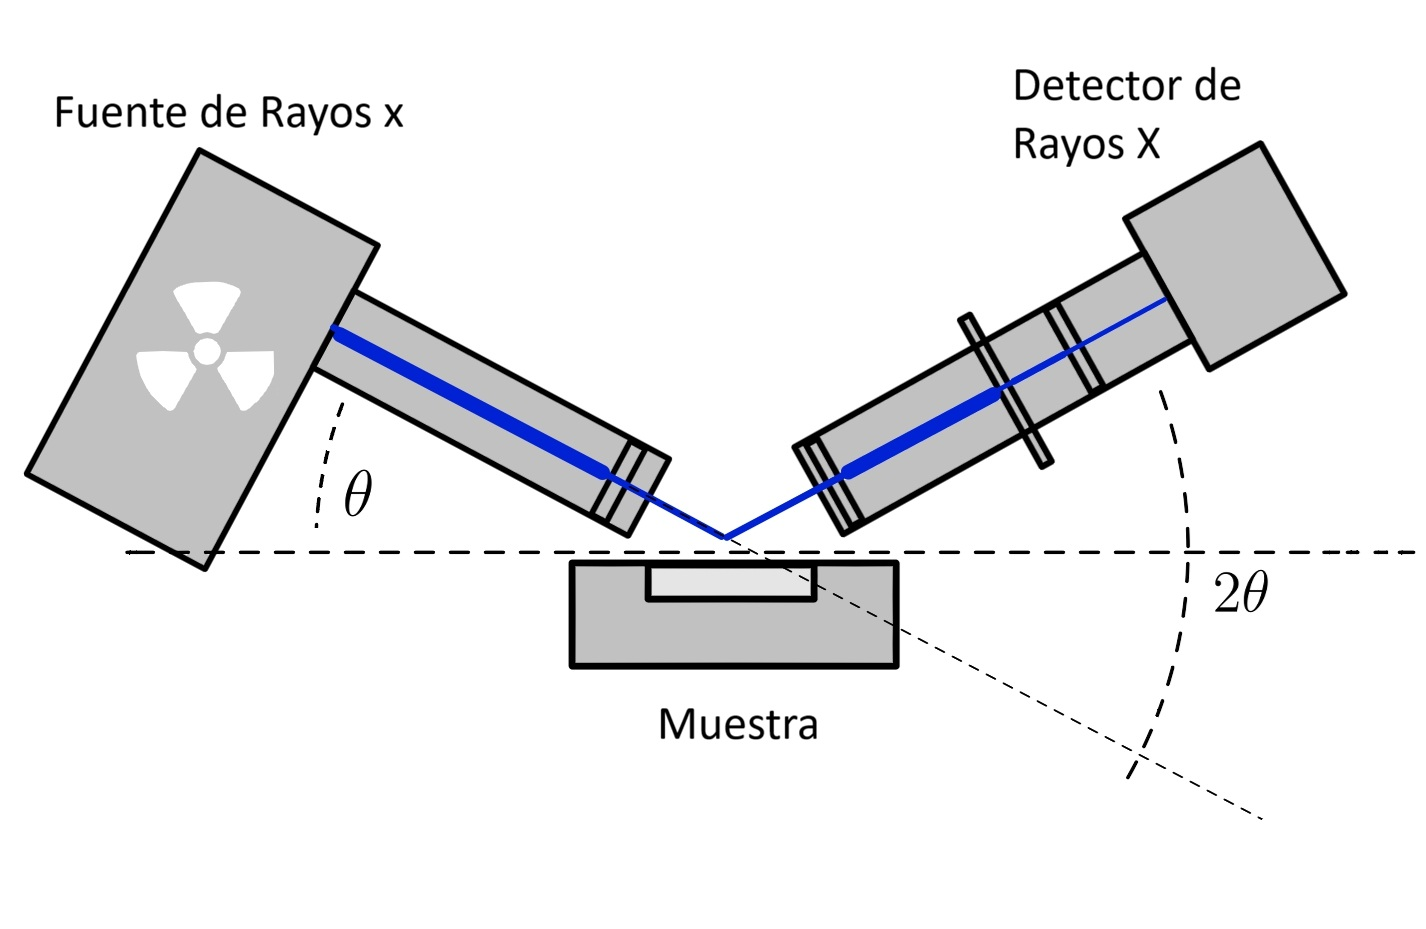
\includegraphics[width=0.5\textwidth]{Imagenes/esquema_difractometro.jpg}
    \caption{Esquema de la geometría Bragg--Brentano en configuración $\theta$--$2\theta$ para el difractómetro de rayos X.}
    \label{fig:bragg-brentano}
\end{figure}

Para la sal de mesa, se realizó un barrido en el rango de $10^\circ < 2\theta < 70^\circ$ con un paso de $0.02^\circ$ y un tiempo de conteo de 2 segundo por paso. Para las sales puras, sus soluciones, la sal \textit{light} y una mezcla con $X_{Br} = 0.6$, se realizó un barrido en el rango de $10^\circ < 2\theta < 80^\circ$ con un paso de $0.02^\circ$ y un tiempo de conteo de 2 segundos por paso.

El difractómetro mide los patrones de difracción irradiando la muestra con rayos X y detectando la intensidad de los rayos difractados en función del ángulo $2\theta$. Estos patrones se utilizan para identificar las fases presentes en la muestra, determinar su estructura cristalina y analizar la composición de las mezclas.

Se utilizó microscopía electrónica de barrido (\textit{SEM}) para observar la morfología de las muestras sólidas obtenidas tras la evaporación. Este análisis permitió evaluar el tamaño y la forma de los cristales formados, así como la presencia de posibles impurezas o defectos en la estructura cristalina.

\section{Resultados}
Se midieron los patrones de difracción de la sal de mesa y la sal \textit{light}, así como también de las soluciones de cloruro de potasio y bromuro de potasio, de estas sales en estado puro y de una mezcla de ambas.

poner aca la sal de mesa y sal light

En las mediciones de las soluciones de KCl y KBr, variando la fracción molar $X_{Br}$ en valores de 0, 0.2, 0.4, 0.6, 0.8 y 1, se observó un desplazamiento progresivo en los picos de intensidad. Inicialmente, los patrones presentan una mayor similitud con el KCl puro, evolucionando gradualmente hacia el perfil del KBr conforme aumenta la concentración de bromo. Este fenómeno se ilustra en la figura \ref{fig:zoom_picos}, donde se aprecia el desplazamiento de los picos de mayor intensidad para cada una de las soluciones analizadas.


\begin{figure}[htbp]
    \centering
    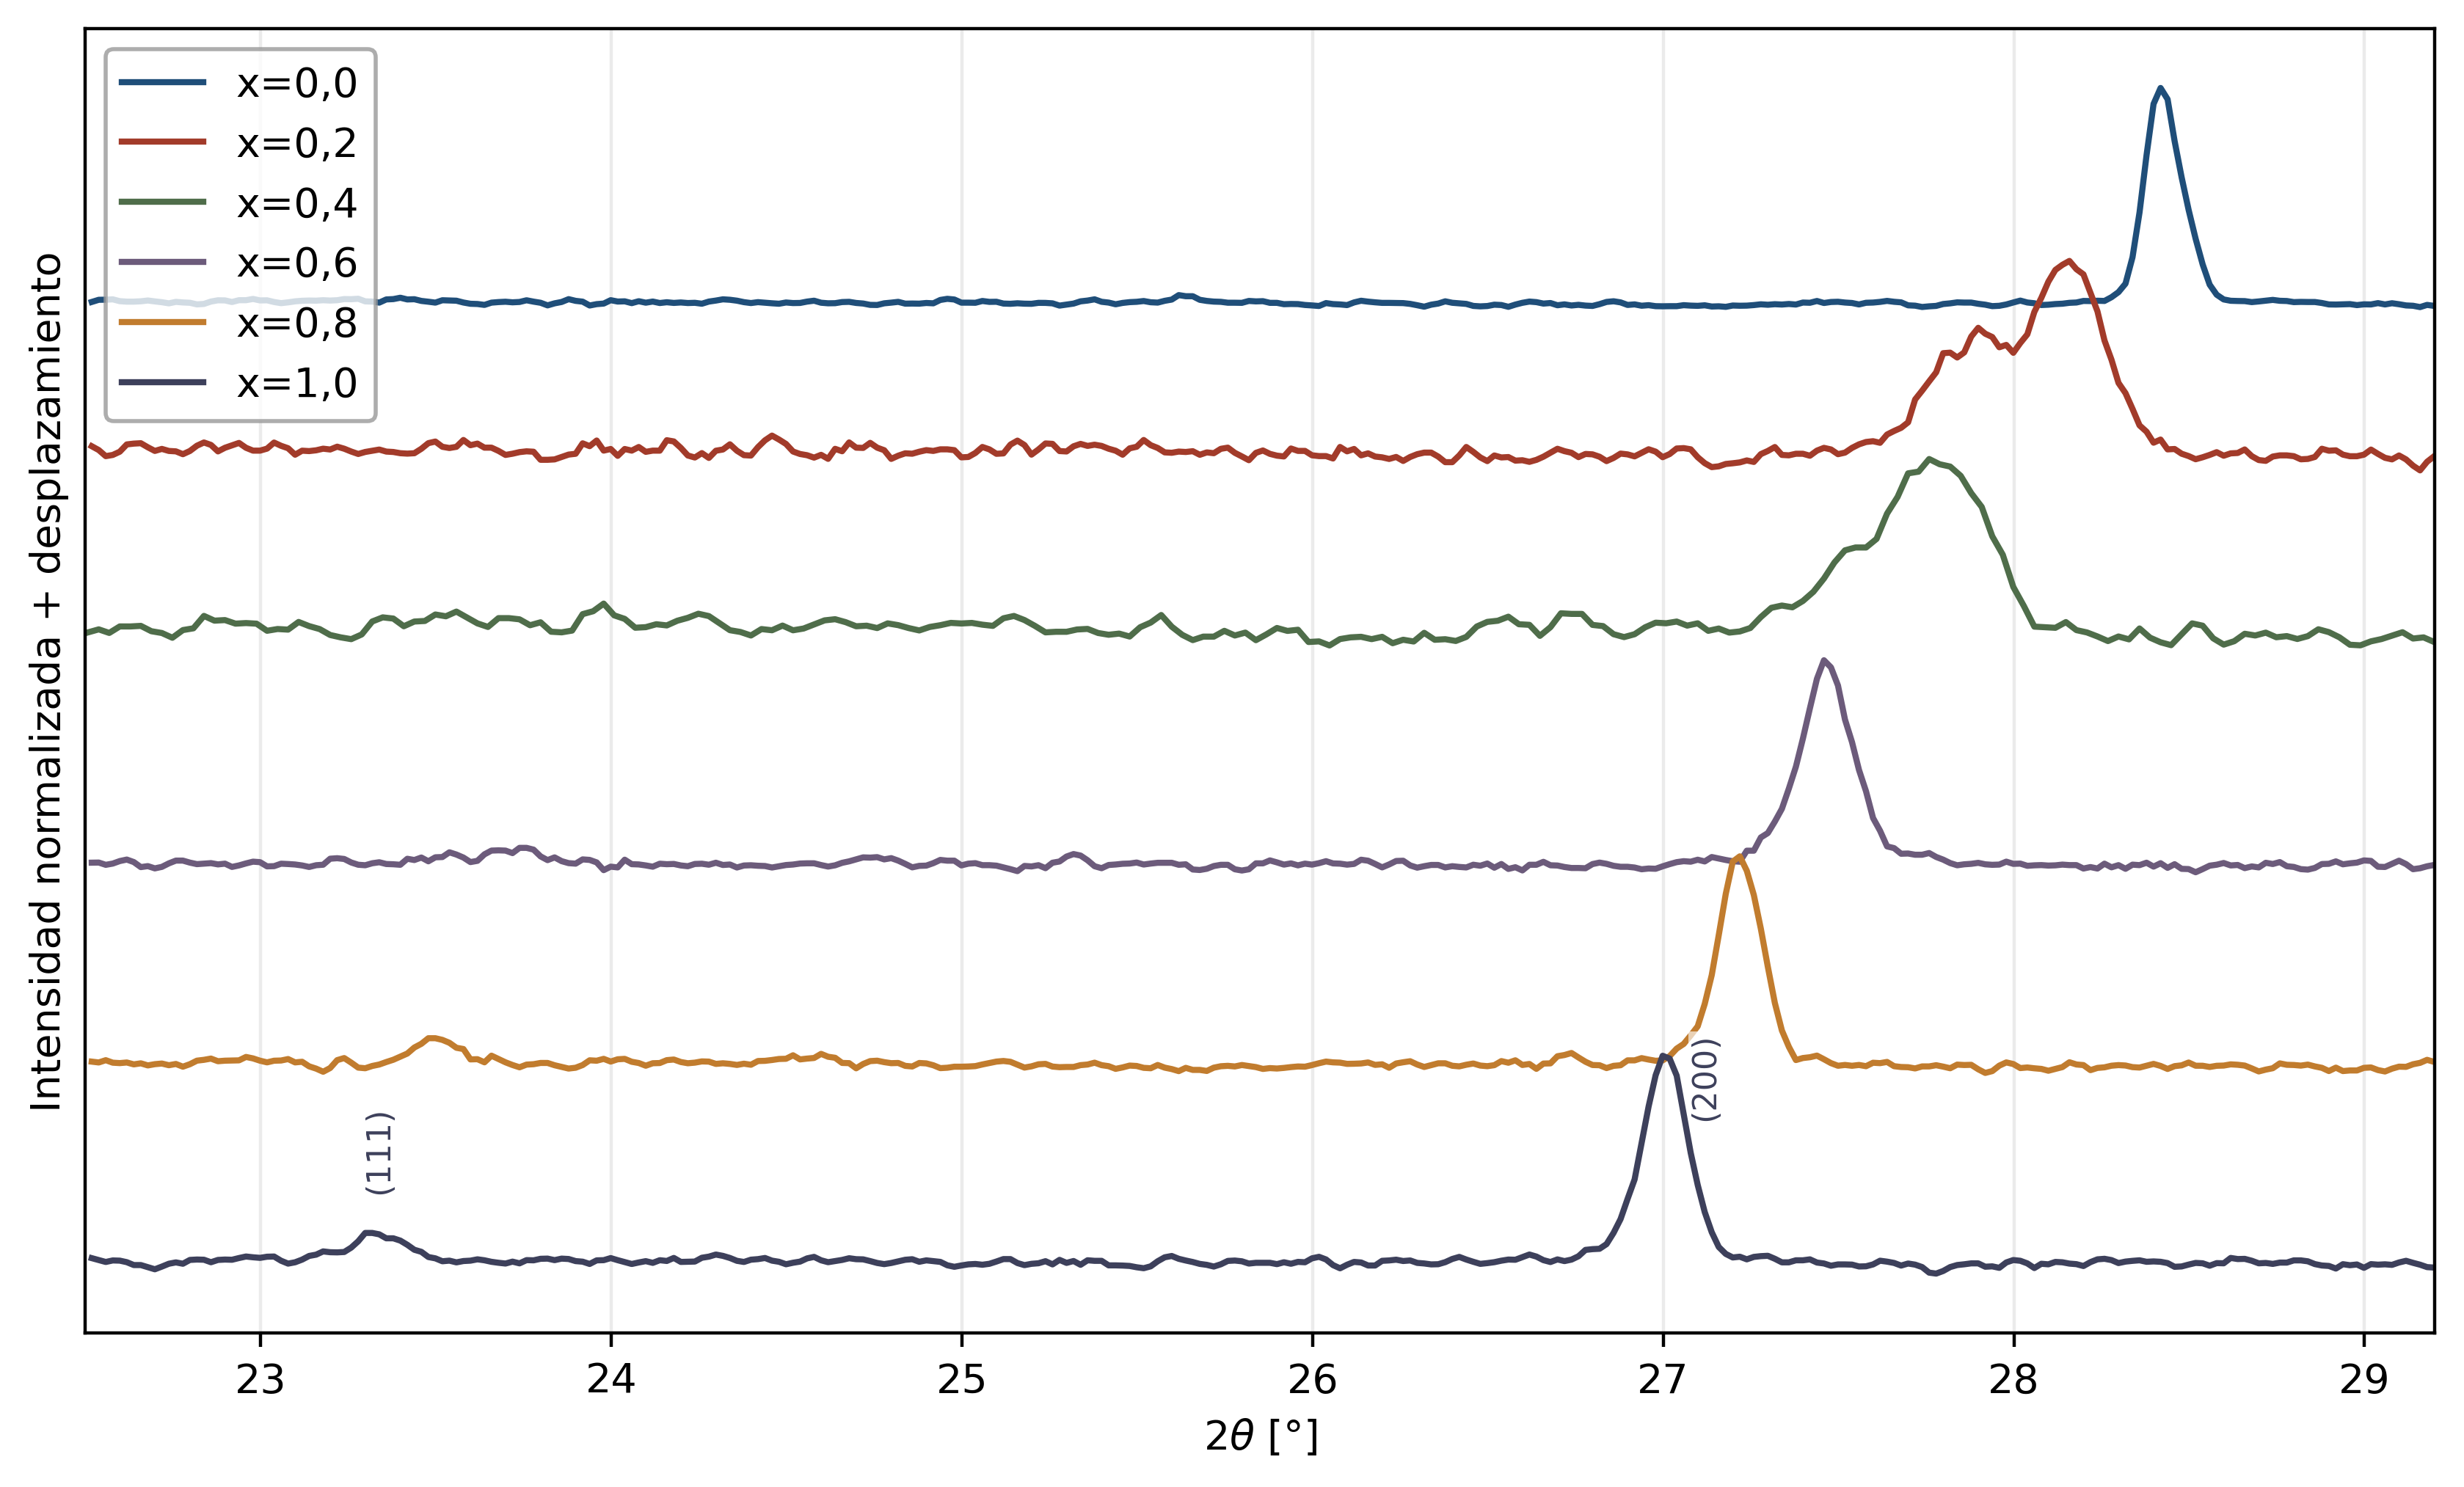
\includegraphics[width=0.5\textwidth]{figuras/zoom_primeros_picos_soluciones.png}
    \caption{Gráfica de los picos de mayor intensidad para cada una de las soluciones analizadas. Donde X representa la fracción molar de KBr en las distintas soluciones.}
    \label{fig:zoom_picos}
\end{figure}


\section{Discusión}
\input{Secciones/Discusion}

\section{Conclusiones}
Pudo verificarse el cumplimiento de la ley de Vegard para soluciones sólidas
$\ce{KCl_{1-x}Br_x}$ al observarse una relación lineal entre los parámetros de red
de dichas soluciones.

Además pudo determinarse los parámetros de red de diferentes compuestos con errores menores
al $0,08\%.$ 

Por otro lado, mediante el uso de difractogramas, se pudo analizar la estructura de diferentes compósitos,
como es el caso de la sal light y del compósito de $\ce{KCl}$ y $\ce{KBr}$ con fracciones molares de $0,4$ y $0,6$ respectivamente.

Luego mediante el uso de un microscopio electrónico de barrido se observó la morfología de las soluciones de $\ce{KCl_{1-x}Br_x},$
observando una mejor cristalización en la muestra que se dejó más tiempo cristalizando.

Finalmente se comprobó que las estructuras de tipo sal de roca son estructuras compactas.

\section*{Referencias}
\renewcommand{\refname}{}

\bibliographystyle{ieeetr}
\bibliography{sources.bib}

\clearpage
% ================== ANEXO: Propagación de errores ==================
\appendix
\input{Secciones/Anexo}

\end{document}
